% Provenance (never printed): see sources/outline_sources.md (Year 3:
% moments of inertia and gravity fields; impact cratering and crater dating;
% volcanism and tectonics on Mars, Venus, Io and the icy moons).
% Brief: sources/book5/BRIEFS.md, ch. 26. Curves from figdata/bachelor-3/
% two_layer_planet.py (two-layer interiors of the Earth, Mars, the Moon and
% Mercury from mean density and moment of inertia) and crater_sfd.py
% (the Ivanov production function and the Hartmann-Neukum chronology of
% Mars from the Craterstats configuration, the lunar chronology of Neukum,
% Hartmann's equilibrium density, and two invented Martian plains whose
% counts are drawn once from a Poisson law). Exercise and problem values in
% the Book 5 scratch calculator calc/ch26.py. Plains A and B are invented.
\chapter{Interiores y superficies planetarias}\label{ch:b3:planetary-interiors-surfaces}

Observada con prismáticos, la Luna tiene dos tipos de terreno. Las brillantes
tierras altas están cubiertas de cráteres, cráter sobre cráter: quedaron saturadas
de cráteres grandes por un bombardeo intenso que terminó hace unos 3.8 mil millones de
años. Los oscuros mares, llanuras rellenas de lava entre hace 4.2 y 1.2
mil millones de años, contienen muchos menos. Las misiones Apolo y Luna
trajeron rocas de ambos, y sus edades radiométricas convirtieron
la densidad de cráteres de una superficie en un reloj. Hoy ese reloj data
llanuras de Marte, Mercurio y las lunas heladas, de las que todavía no se ha
traído ninguna roca. Este capítulo lee los interiores de los planetas en su
gravedad, rotación y mareas, y luego sus superficies en sus cráteres,
volcanes y fallas.
% ledger: french:highlands, nasa:moon-core, marchi:neukum

\begin{recall}
El factor de momento de inercia $C = I/MR^2$, el modelo de dos capas de un planeta
construido a partir de él y de la densidad media, los planetas terrestres y los
gigantes están en el volumen de primer año, en su capítulo de planetología
comparada; las plumas del manto y las grandes provincias ígneas, en su capítulo sobre
puntos calientes. La diferenciación planetaria y los meteoritos están en el volumen de
segundo año, en su capítulo sobre formación planetaria. El \omterm{def:b3:gravity-geodesy:j2}{factor de forma dinámico}
$J_2$, la \omterm{thm:b3:gravity-geodesy:maccullagh}{fórmula de MacCullagh} y la flexión de la litosfera están en este
volumen, en su capítulo sobre gravedad y geodesia; el \omterm{def:b3:mantle-convection:rayleigh}{número de Rayleigh}, en su
capítulo sobre convección del manto. Las mareas, las leyes de Kepler y los módulos
elásticos están en los libros de física; la distribución de Poisson, en los
libros de matemáticas.
\end{recall}

\section{Interiores a partir de la gravedad, la rotación y las mareas}\label{sec:b3:planetary-interiors-surfaces:interiors}

La masa de un planeta, obtenida a partir de la órbita de una luna o de una sonda, da
su densidad media; la precesión de su eje y su $J_2$ dan su momento de
inercia. La proposición de dos capas del volumen de primer año convierte los dos
números en un núcleo, pero solo una vez elegida una densidad para el manto: dos
medidas no pueden fijar tres incógnitas.

\begin{omfigure}
\centering
\begin{tikzpicture}
\begin{axis}[width=0.78\linewidth, height=0.46\linewidth,
  xmin=3000, xmax=16000, ymin=0, ymax=1,
  xlabel={densidad del núcleo $\rho_c$ (\unit{kg.m^{-3}})},
  ylabel={radio del núcleo / radio del planeta $x$},
  tick label style={font=\scriptsize}, label style={font=\small},
  scaled x ticks=false, xtick={4000,6000,8000,10000,12000,14000,16000},
  xticklabels={4000,6000,8000,10\,000,12\,000,14\,000,16\,000}]
\addplot[thick, omDef] table[x=rho_c, y=x] {figdata/out/bachelor-3-two_layer_planet-curve-Earth.dat};
\addplot[thick, red!70!black] table[x=rho_c, y=x] {figdata/out/bachelor-3-two_layer_planet-curve-Mars.dat};
\addplot[thick, black!60, dashed] table[x=rho_c, y=x] {figdata/out/bachelor-3-two_layer_planet-curve-Moon.dat};
\addplot[thick, orange!80!black] table[x=rho_c, y=x] {figdata/out/bachelor-3-two_layer_planet-curve-Mercury.dat};
\addplot[only marks, mark=*, mark size=2pt, black] table[x=rho_c, y=x] {figdata/out/bachelor-3-two_layer_planet-points.dat};
\node[font=\scriptsize, omDef, anchor=south west] at (axis cs:12600,0.55) {Tierra};
\node[font=\scriptsize, red!70!black, anchor=south west] at (axis cs:6600,0.55) {Marte};
\node[font=\scriptsize, black!70, anchor=south west] at (axis cs:11000,0.2) {Luna};
\node[font=\scriptsize, orange!80!black, anchor=south west] at (axis cs:7300,0.83) {Mercurio};
\end{axis}
\end{tikzpicture}
\par\smallskip{\small Los modelos de dos capas permitidos por la densidad media y el
factor de momento de inercia de cuatro cuerpos: cada curva recorre las
posibles densidades del manto, de modo que un manto más denso deja un núcleo más pequeño y más denso.
Los puntos marcan los radios medidos del núcleo: el de la Tierra, a partir de la sismología;
el de Marte, a partir del sismómetro de InSight; el núcleo interno y la
capa líquida de la Luna; y el de Mercurio, a partir del campo gravitatorio de la
sonda MESSENGER.}\label{fig:b3:planetary-interiors-surfaces:two-layer}
\end{omfigure}
% ledger: planet:Earth.density, planet:Mars.density, planet:Moon.density, planet:Mercury.density, earth:MoI, nasa:mars, nasa:moon, nasa:mercury, data:prem, jpl:insight-interior, nasa:moon-core, agu:mercury-core

Cada planeta da una curva, no un punto. Para Marte, el radio del núcleo de
\qty{1830}{km} medido por InSight fija un manto de \qty{3460}{kg.m^{-3}}
y un núcleo de \qty{6460}{kg.m^{-3}}. Para Mercurio, el núcleo de unos
\qty{2000}{km} de radio ocupa el 82~por ciento del radio. La curva de la Luna es
casi plana: su $C = 0.394$ está tan cerca de $\tfrac25$ que encaja un núcleo pequeño
de cualquier densidad, y un cambio de $0.001$ en $C$ desplaza el radio del núcleo
más de un factor dos (véase el \cref{exo:b3:planetary-interiors-surfaces:10}).
La gravedad por sí sola no permite ver un núcleo pequeño; sí lo permiten las mareas y las ondas sísmicas.
% ledger: jpl:insight-interior, agu:mercury-core, nasa:moon

\begin{definition}[número de Love]\label{def:b3:planetary-interiors-surfaces:love-number}
Cuando un potencial de marea de grado~2 actúa sobre un planeta, este se deforma y
su masa redistribuida añade un potencial propio. El \emph{número
de Love}\index{número de Love} $k_2$ es la razón entre ese potencial añadido y
el potencial de marea, ambos tomados en la superficie del planeta.
\end{definition}

Un planeta rígido tiene $k_2 = 0$; un planeta fluido de densidad uniforme cede
por completo, con $k_2 = \tfrac32$. Entre ambos extremos, el número mide
cuánta parte del planeta cede.

\begin{proposition}[Número de Love de una esfera elástica uniforme]\label{prop:b3:planetary-interiors-surfaces:kelvin}
Una esfera incompresible de densidad uniforme $\rho$, radio $R$, gravedad superficial
$g$ y rigidez $\mu$ tiene
\[
  k_2 = \frac{3/2}{1 + \dfrac{19\mu}{2\rho g R}} .
\]
\end{proposition}

El resultado, debido a Kelvin, se admite. La razón $\mu/\rho gR$ compara
la rigidez elástica con la autogravedad que devuelve el abultamiento de marea
a su posición: los planetas pequeños son rígidos, los grandes ceden. Para Marte, $\rho gR =
\qty{4.97e10}{Pa}$; con la rigidez del manto superior terrestre,
\qty{67}{GPa} a \qty{80}{km} de profundidad en el modelo de Tierra de referencia, la
fórmula da $k_2 = 0.109$. El seguimiento de la sonda en órbita Mars Global Surveyor
midió la marea solar de Marte: $k_2 = 0.153 \pm 0.017$, demasiado
grande para un núcleo de hierro sólido. Al menos la parte exterior del núcleo es
líquida, y en 2003 se situó su radio entre 1520 y \qty{1840}{km}.
% ledger: nasa:mars, const:G, data:prem, yoder:mars-k2

Los sismómetros zanjaron la cuestión. El módulo de aterrizaje InSight registró
terremotos marcianos y detectó ondas reflejadas en la parte superior del núcleo: radio
\qty{1830}{km}, bajo un manto de \qty{1560}{km} de profundidad y una corteza de 20 a
\qty{37}{km} de espesor. En la Luna, los sismómetros instalados por los astronautas
del Apolo registraron seísmos lunares, los más profundos de ellos, a cientos de
kilómetros bajo la superficie, provocados por las mareas terrestres. El núcleo lunar
se describe hoy como un núcleo interno sólido rico en hierro de \qty{240}{km} de radio,
una capa líquida de hierro de \qty{90}{km} de espesor que lo rodea y una
capa parcialmente fundida por encima.
% ledger: jpl:insight-interior, nasa:moonquakes, nasa:moon-core

\section{Impacto y cráteres}\label{sec:b3:planetary-interiors-surfaces:impacts}

Un cuerpo procedente del espacio impacta contra un planeta a una velocidad no inferior
a la de escape del planeta, \qty{11.2}{km.s^{-1}} en el caso de la Tierra; los asteroides
suelen encontrarse con la Tierra a una velocidad de entre 15 y \qty{25}{km.s^{-1}}, y los
cometas, de hasta \qty{60}{km.s^{-1}}. A \qty{20}{km.s^{-1}}, cada kilogramo transporta
\qty{2e8}{J}, unas cincuenta veces la energía de un kilogramo de explosivo. El
impacto envía una onda de choque al terreno y al proyectil, que
se funde y se vaporiza; detrás del choque, la roca se pone en movimiento hacia afuera y
en cuestión de segundos se abre un cráter.
% ledger: french:velocities, french:table21

\begin{definition}[Cráter transitorio, cráter simple, cráter complejo, manto de eyecta]\label{def:b3:planetary-interiors-surfaces:crater-morphology}
El \emph{cráter transitorio}\index{cráter transitorio} es la cavidad en forma de cuenco
abierta por el flujo de excavación en el momento en que deja de crecer; su
profundidad es de aproximadamente un tercio de su diámetro. Un \emph{cráter
simple}\index{cráter simple} es un cuenco con un borde elevado, con el cráter
transitorio apenas modificado: sus paredes empinadas se derrumban hacia dentro formando
una lente de brecha. Un \emph{cráter complejo}\index{cráter complejo} es un cráter
más grande cuyo cuenco transitorio colapsó: el suelo se elevó formando un levantamiento
central, el borde se deslizó hacia dentro a lo largo de terrazas y el suelo es plano. El \emph{manto de
eyecta}\index{manto de eyecta} es la capa de roca excavada que se
proyecta más allá del borde y se deposita alrededor del cráter.
\end{definition}
% ledger: french:transient, french:transition

\begin{omfigure}
\centering
\begin{tikzpicture}[x=0.55cm, y=0.55cm, font=\scriptsize, >=stealth]
\def\simpleprofile{(-6,0) -- (-3.6,0) .. controls (-3.0,0.45) .. (-2.6,0.55) .. controls (-1.8,-2.6) and (1.8,-2.6) .. (2.6,0.55) .. controls (3.0,0.45) .. (3.6,0) -- (6,0)}
\def\complexprofile{(-7,0) -- (-5.4,0) -- (-4.6,0.5) -- (-4.0,-0.3) -- (-3.6,-0.25) -- (-3.1,-1.0) -- (-2.7,-0.95) -- (-2.3,-1.5) -- (-0.8,-1.5) -- (-0.5,-0.6) -- (0,-0.3) -- (0.5,-0.6) -- (0.8,-1.5) -- (2.3,-1.5) -- (2.7,-0.95) -- (3.1,-1.0) -- (3.6,-0.25) -- (4.0,-0.3) -- (4.6,0.5) -- (5.4,0) -- (7,0)}
\begin{scope}
\fill[black!8] \simpleprofile -- (6,-4) -- (-6,-4) -- cycle;
\begin{scope}
\clip \simpleprofile -- (6,-4) -- (-6,-4) -- cycle;
\draw[black!45] (-6,-1.2) -- (6,-1.2) (-6,-2.4) -- (6,-2.4);
\fill[black!28] (-2.25,-0.5) .. controls (-1.2,-2.05) and (1.2,-2.05) .. (2.25,-0.5) .. controls (1.0,-0.8) and (-1.0,-0.8) .. (-2.25,-0.5);
\end{scope}
\fill[black!40] (-5.2,0) -- (-2.6,0.55) -- (-3.6,0.12) -- cycle;
\fill[black!40] (5.2,0) -- (2.6,0.55) -- (3.6,0.12) -- cycle;
\draw[thick] \simpleprofile;
\draw[omDef, dashed, thick] (-2.4,0.35) .. controls (-1.6,-3.1) and (1.6,-3.1) .. (2.4,0.35);
\node[anchor=south] at (0,1.2) {cráter simple};
\node[fill=black!28, inner sep=1pt] at (0,-1.45) {lente de brecha};
\node[omDef, anchor=north, fill=black!8, inner sep=1pt] at (0,-2.65) {cráter transitorio};
\draw[->] (-4.9,1.2) node[anchor=south] {eyecta} -- (-4.3,0.2);
\draw[->] (3.6,1.4) node[anchor=south] {borde elevado} -- (2.8,0.62);
\end{scope}
\begin{scope}[xshift=7.6cm]
\fill[black!8] \complexprofile -- (7,-4) -- (-7,-4) -- cycle;
\begin{scope}
\clip \complexprofile -- (7,-4) -- (-7,-4) -- cycle;
\draw[black!45] (-7,-1.2) -- (7,-1.2);
\draw[black!45] (-7,-2.4) -- (-1.3,-2.4) .. controls (-0.6,-2.4) and (-0.5,-1.75) .. (0,-1.75) .. controls (0.5,-1.75) and (0.6,-2.4) .. (1.3,-2.4) -- (7,-2.4);
\draw[black!45] (-7,-3.4) -- (-1.6,-3.4) .. controls (-0.7,-3.4) and (-0.6,-2.7) .. (0,-2.7) .. controls (0.6,-2.7) and (0.7,-3.4) .. (1.6,-3.4) -- (7,-3.4);
\draw[black!70] (-4.0,-0.3) -- (-3.2,-2.0) (4.0,-0.3) -- (3.2,-2.0) (-3.1,-1.0) -- (-2.5,-2.2) (3.1,-1.0) -- (2.5,-2.2);
\end{scope}
\draw[thick] \complexprofile;
\node[anchor=south] at (0,1.5) {cráter complejo};
\draw[->] (1.4,0.75) node[anchor=south west, inner sep=1pt] {levantamiento central} -- (0.25,-0.2);
\node[anchor=north, fill=black!8, inner sep=0.5pt] at (-1.3,-1.6) {suelo plano};
\draw[->] (-3.2,1.4) node[anchor=south] {terrazas} -- (-3.8,-0.12);
\draw[->] (-5.6,-0.6) node[anchor=east, fill=black!8, inner sep=1pt, xshift=4pt] {fallas} -- (-3.65,-1.35);
\node[anchor=north, fill=black!8, inner sep=1pt] at (0,-3.55) {capas levantadas};
\end{scope}
\end{tikzpicture}
\par\smallskip{\small Secciones transversales de un \omterm{def:b3:planetary-interiors-surfaces:crater-morphology}{cráter simple} y de un \omterm{def:b3:planetary-interiors-surfaces:crater-morphology}{cráter complejo} en
roca estratificada (no a escala). A la izquierda: el cuenco de un \omterm{def:b3:planetary-interiors-surfaces:crater-morphology}{cráter simple} conserva la
forma del \omterm{def:b3:planetary-interiors-surfaces:crater-morphology}{cráter transitorio} (discontinuo), parcialmente rellena por una lente de brecha,
bajo un borde elevado y un \omterm{def:b3:planetary-interiors-surfaces:crater-morphology}{manto de eyecta}. A la derecha: en un \omterm{def:b3:planetary-interiors-surfaces:crater-morphology}{cráter complejo} el
cuenco transitorio ha colapsado; las capas profundas se han elevado bajo un levantamiento
central, y el borde se ha deslizado hacia dentro a lo largo de fallas hasta
terrazas.}\label{fig:b3:planetary-interiors-surfaces:craters}
\end{omfigure}
% ledger: french:transient, french:transition

\begin{omfigure}
\centering
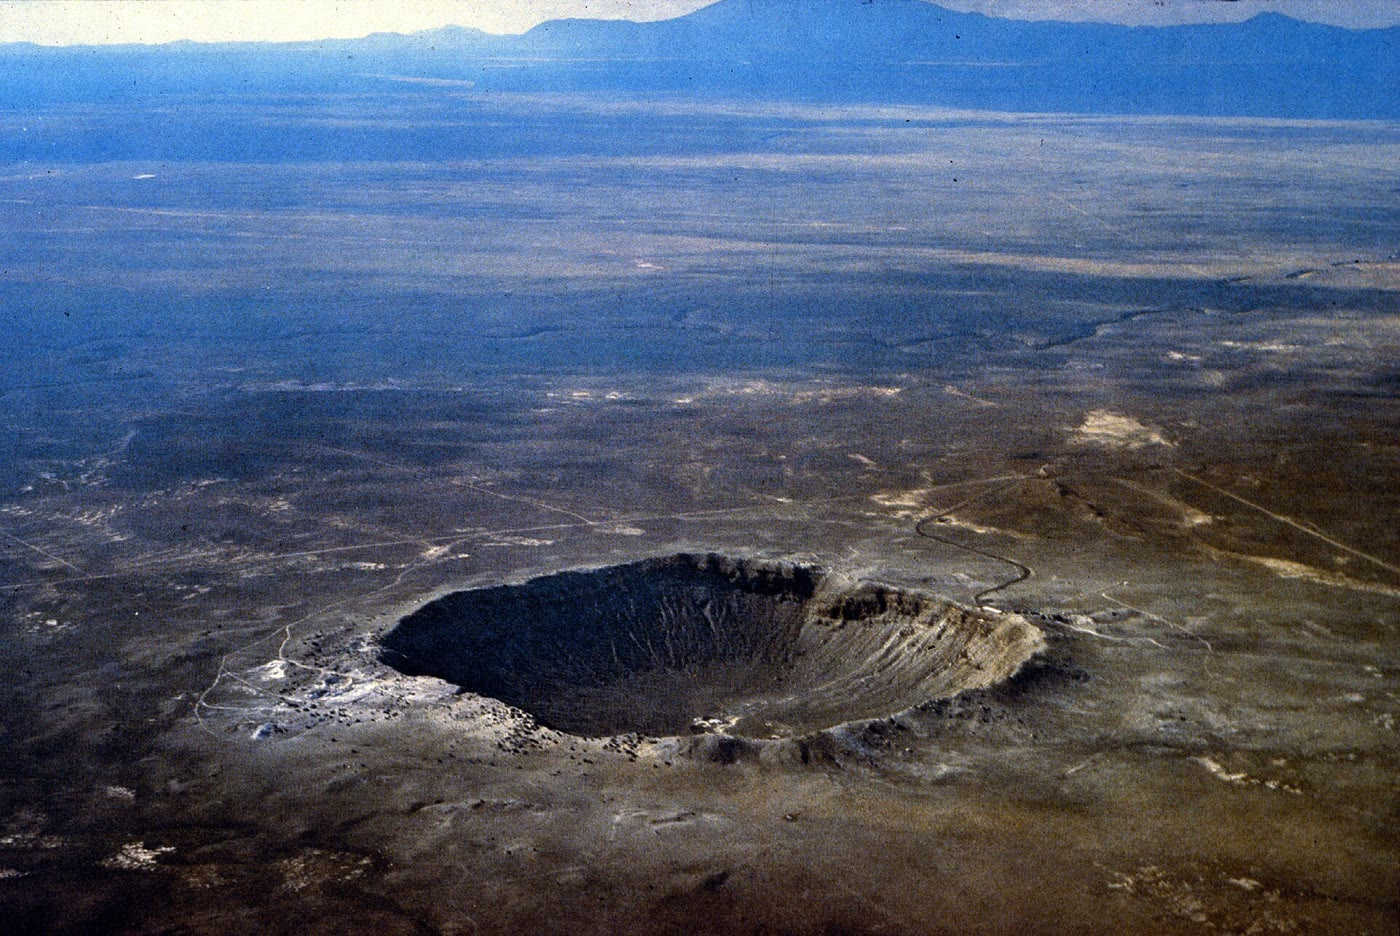
\includegraphics[width=0.66\linewidth]{images/book5/b3-barringer-crater.jpg}
\par\smallskip{\small Cráter Barringer, Arizona, un \omterm{def:b3:planetary-interiors-surfaces:crater-morphology}{cráter simple}
de \qty{1.2}{km} de diámetro, formado hace unos 50\,000 años por un meteorito de hierro
de unos \qty{30}{m} de diámetro; el borde se alza sobre la meseta y el \omterm{def:b3:planetary-interiors-surfaces:crater-morphology}{manto de eyecta}
se extiende a su alrededor. Fotografía aérea, USGS/D.~Roddy, dominio
público.}\label{fig:b3:planetary-interiors-surfaces:barringer}
\end{omfigure}
% ledger: photo:b3-barringer, french:barringer

La excavación de un cráter de \qty{1}{km} de diámetro dura unos seis segundos; la de un
cráter de \qty{200}{km}, alrededor de un minuto y medio. El tamaño del
cráter que produce un impacto depende de la energía del proyectil, de la gravedad y
de la resistencia de la roca; las leyes que relacionan estas magnitudes se ajustan a
experimentos y explosiones en forma de productos de grupos adimensionales,
y se admiten aquí. Su espíritu reside en un balance de energías.
% ledger: french:transient

\begin{proposition}[Escalado en el régimen gravitatorio]\label{prop:b3:planetary-interiors-surfaces:scaling}
Si una fracción fija de la energía del impacto $E$ levanta la roca excavada de
densidad $\rho$ frente a la gravedad $g$, el diámetro del cráter crece como
\[
  D \propto \left(\frac{E}{\rho g}\right)^{1/4} .
\]
\end{proposition}

\begin{proof}
El volumen excavado escala como $D^3$, su masa como $\rho D^3$, y se
eleva a una altura del orden de $D$: el trabajo es del orden de $\rho g D^4$, que
es proporcional a $E$.
\end{proof}

Parte de la energía se invierte en calor, en fusión y en la rotura de la roca, de modo que
las leyes reales quedan entre esta y reglas más simples: una tabla citada a menudo
para la Tierra da un cráter veinte veces más ancho que su
proyectil pétreo. La gravedad también determina dónde un cráter deja de ser simple. Las
paredes del cuenco transitorio colapsan cuando el peso de la roca que sostienen,
del orden de $\rho g D/3$, supera la resistencia de la roca, de modo que el
diámetro de transición varía como $1/g$: unos \qty{4}{km} en roca cristalina y
\qty{2}{km} en sedimentos en la Tierra, unos \qty{20}{km} en la
Luna, donde la gravedad es seis veces menor.
% ledger: french:table21, french:transition, planet:Earth.gravity, planet:Moon.gravity

\section{Datación por cráteres}\label{sec:b3:planetary-interiors-surfaces:dating}

Una superficie que se deja sin alterar acumula cráteres al ritmo con que los cuerpos
la impactan. Contarlos permite datar la superficie, siempre que se conozca el ritmo y los
cráteres sean los de la superficie, no los de lo que yace debajo ni los de los
escombros lanzados desde un vecino.

\begin{definition}[Distribución de tamaño--frecuencia de cráteres]\label{def:b3:planetary-interiors-surfaces:sfd}
La \emph{distribución de tamaño--frecuencia de cráteres}\index{distribución de tamaño--frecuencia de cráteres}
de una superficie es el número $N(D)$ de cráteres de diámetro igual o mayor que $D$ por
unidad de área, en función de $D$ (la distribución acumulada), o bien los
números contados en intervalos de diámetro, por lo general cada uno $\sqrt2$ veces más ancho que
el anterior (la distribución incremental).
\end{definition}

\begin{definition}[Datación por cráteres; funciones de producción y de cronología; densidad de equilibrio]\label{def:b3:planetary-interiors-surfaces:crater-dating}
La \emph{datación por cráteres}\index{datación por cráteres} es la determinación de la edad
de una superficie a partir de la densidad de sus cráteres. La \emph{función de producción
de cráteres}\index{función de producción de cráteres} es la forma de la
distribución de tamaño--frecuencia de los cráteres que adquiere una superficie, $F(D) =
N(D)/N(\qty{1}{km})$, supuesta la misma a cada edad. La \emph{función de
cronología de cráteres}\index{función de cronología de cráteres} $N_1(T)$ es el
número de cráteres de \qty{1}{km} o más por unidad de área acumulados en un
tiempo $T$. Una superficie se halla en la \emph{densidad de equilibrio
de cráteres}\index{densidad de equilibrio de cráteres} para los cráteres de un tamaño dado
cuando cada nuevo cráter borra, por término medio, tantos antiguos como añade:
su número ya no crece.
\end{definition}

La edad modelo de una superficie se deduce de un único recuento: $N(D)$ medido para cualquier
$D$ da $N_1 = N(D)/F(D)$, y $T$ resuelve $N_1(T) = N_1$. Las rectas
$N(D) = N_1(T)F(D)$ para $T$ fijo se llaman isócronas. Para Marte, una función de producción muy
utilizada es un polinomio de grado~11 en $\log_{10}D$, y la
función de cronología tiene la forma
\[
  N_1(T) = a\left(e^{bT} - 1\right) + cT , \qquad
  a = \qty{3.22e-14}{km^{-2}}, \ b = \qty{6.93}{Ga^{-1}}, \
  c = \qty{4.875e-4}{km^{-2}.Ga^{-1}} ,
\]
lineal durante los últimos tres mil millones de años, y marcadamente exponencial antes. La
función de la Luna tiene la misma forma, con $a = \num{5.44e-14}$ y $c =
\num{8.38e-4}$. Se ajustó a las edades de los emplazamientos de aterrizaje de las misiones Apolo y
Luna; la de Marte es la de la Luna, escalada por una estimación de la razón entre
los ritmos de formación de cráteres en Marte y en la Luna.
% ledger: craterstats:mars-pf, craterstats:mars-cf, craterstats:moon-cf, marchi:neukum

\begin{omfigure}
\centering
\begin{tikzpicture}
\begin{groupplot}[group style={group size=2 by 1, horizontal sep=1.6cm},
  width=0.48\linewidth, height=0.46\linewidth,
  tick label style={font=\scriptsize}, label style={font=\small}, title style={font=\small}]
\nextgroupplot[title={isócronas en Marte}, xmode=log, ymode=log, xmin=0.1, xmax=100,
  ymin=1e-8, ymax=100, xlabel={diámetro del cráter $D$ (\unit{km})},
  ylabel={$N(D)$, cráteres $\geq D$ por \unit{km^2}},
  xtick={0.1,1,10,100}, xticklabels={0.1,1,10,100},
  ytick={1e-8,1e-6,1e-4,1e-2,1}]
\addplot[thick, black!50, dashed] table[x=D, y=eq] {figdata/out/bachelor-3-crater_sfd-iso.dat};
\addplot[omDef] table[x=D, y=N_0.1] {figdata/out/bachelor-3-crater_sfd-iso.dat};
\addplot[omDef] table[x=D, y=N_1] {figdata/out/bachelor-3-crater_sfd-iso.dat};
\addplot[omDef] table[x=D, y=N_3.5] {figdata/out/bachelor-3-crater_sfd-iso.dat};
\addplot[red!70!black, thick] table[x=D, y=N_4] {figdata/out/bachelor-3-crater_sfd-iso.dat};
\node[font=\tiny, omDef, anchor=north east] at (axis cs:0.75,8e-6) {0.1~Ga};
\node[font=\tiny, omDef, anchor=north east] at (axis cs:2.6,1e-5) {1~Ga};
\node[font=\tiny, omDef, anchor=north east] at (axis cs:9,3.5e-5) {3.5~Ga};
\node[font=\tiny, red!70!black, anchor=north east] at (axis cs:45,2.5e-5) {4~Ga};
\node[font=\tiny, black!60, anchor=south, rotate=-30] at (axis cs:25,3.5e-4) {equilibrio};
\nextgroupplot[title={funciones de cronología}, ymode=log, xmin=0, xmax=4.5,
  ymin=1e-5, ymax=0.3, xlabel={edad $T$ (\unit{Ga})}, ylabel={$N_1$ por \unit{km^2}},
  legend style={font=\scriptsize, at={(0.03,0.97)}, anchor=north west}]
\addplot[thick, red!70!black] table[x=T, y=mars] {figdata/out/bachelor-3-crater_sfd-chron.dat};
\addlegendentry{Marte}
\addplot[thick, black!60, dashed] table[x=T, y=moon] {figdata/out/bachelor-3-crater_sfd-chron.dat};
\addlegendentry{Luna}
\end{groupplot}
\end{tikzpicture}
\par\smallskip{\small Izquierda: isócronas de Marte, las densidades acumuladas de
cráteres en superficies de 0.1, 1, 3.5 y 4 mil millones de años, con la
densidad de equilibrio (discontinua), que limita todo recuento: en una superficie de 4
mil millones de años los cráteres menores de unos \qty{0.7}{km} están en
equilibrio y ya no registran la edad. Derecha: las funciones de cronología
de Marte y de la Luna, el número de cráteres de \qty{1}{km} o más por
kilómetro cuadrado frente a la edad de la
superficie.}\label{fig:b3:planetary-interiors-surfaces:sfd}
\end{omfigure}
% ledger: craterstats:mars-pf, craterstats:mars-cf, craterstats:moon-cf, craterstats:equilibrium

Los cráteres se forman al azar, de forma independiente unos de otros, de modo que el número
$n$ hallado en un área es una variable de Poisson.

\begin{proposition}[Error de conteo de una edad modelo]\label{prop:b3:planetary-interiors-surfaces:poisson}
Si se cuentan $n$ cráteres en un área $A$, la densidad $N = n/A$ tiene la
desviación típica $\sqrt n/A$, un error relativo $1/\sqrt n$, y la edad modelo
la desviación típica
\[
  \sigma_T = \frac{N_1(T)}{\sqrt n\,N_1'(T)} .
\]
\end{proposition}

\begin{proof}
Una variable de Poisson de media $\lambda$ tiene varianza $\lambda$, estimada mediante
$n$. La edad es $T = N_1^{-1}(N_1)$; a primer orden $\sigma_T =
\sigma_{N_1}/N_1'(T)$, y $\sigma_{N_1} = N_1/\sqrt n$.
\end{proof}

El error relativo del recuento por sí solo es del diez por ciento para cien
cráteres. En una superficie joven, donde $N_1$ es lineal, la edad hereda ese error:
$\sigma_T/T = 1/\sqrt n$. En una antigua, la función empinada lo reduce, en
un factor de seis a \qty{3.8}{Ga} (el \cref{exo:b3:planetary-interiors-surfaces:11});
las edades modelo de las superficies antiguas quedan entonces limitadas por la calibración
de la propia función. Dos límites más acotan un recuento. Los cráteres pequeños
se saturan: en las superficies más antiguas, los cráteres por debajo de unos \qty{0.7}{km} están en
la densidad de equilibrio y dejan de registrar el tiempo. Y una superficie puede renovarse
sin borrarse del todo: una colada de lava que sepulta los cráteres pequeños pero no los
bordes de los grandes deja una distribución con un quiebro, antigua en $D$ grande y
joven en $D$ pequeño. El quiebro data la \omterm{def:b3:planetary-interiors-surfaces:resurfacing}{renovación de la superficie}.
% ledger: craterstats:equilibrium

\begin{definition}[Renovación de la superficie]\label{def:b3:planetary-interiors-surfaces:resurfacing}
La \emph{renovación de la superficie}\index{renovación de la superficie} es la renovación de una
superficie planetaria, por lava, sedimento, hielo o deformación, que elimina o sepulta sus
cráteres y reinicia su reloj de cráteres.
\end{definition}

\section{Volcanismo y tectónica más allá de la Tierra}\label{sec:b3:planetary-interiors-surfaces:volcanism}

Todo planeta terrestre pierde su calor interno a través de su litosfera.
La Tierra lo hace con placas móviles; los demás, de otra manera.

\begin{definition}[Tapa estancada]\label{def:b3:planetary-interiors-surfaces:stagnant-lid}
Un planeta tiene una \emph{tapa estancada}\index{tapa estancada} cuando su litosfera
es una única cáscara rígida que no participa en la convección del
manto subyacente: el calor la atraviesa por conducción y por el magma que asciende
a través de ella. En un planeta de tapa móvil, como la Tierra, la litosfera está
fragmentada en placas que se hunden de nuevo en el manto.
\end{definition}

\begin{definition}[Vulcanismo de tubo de calor]\label{def:b3:planetary-interiors-surfaces:heat-pipe}
El \emph{vulcanismo de tubo de calor}\index{vulcanismo de tubo de calor} es la pérdida de
calor interno de un planeta sobre todo por el ascenso de magma a través de conductos estrechos y
su erupción en la superficie, donde las lavas se enfrían y quedan sepultadas por otras
posteriores: la litosfera se construye desde arriba y es arrastrada hacia abajo, fría.
\end{definition}

\begin{omfigure}
\centering
\begin{tikzpicture}[x=0.5cm, y=0.5cm, font=\scriptsize, >=stealth]
\foreach \dx/\name in {0/tapa móvil, 9.5/tapa estancada, 19/tubo de calor} {
  \begin{scope}[xshift=\dx*0.5cm]
  \fill[orange!15] (0,0) rectangle (8,4);
  \node[anchor=south] at (4,5.6) {\name};
  \end{scope}}
% mobile lid: plates, ridge, slab
\fill[omDef!35] (0,4) rectangle (3.9,4.8);
\fill[omDef!35] (4.1,4) rectangle (6.2,4.8);
\fill[omDef!35] (6.2,4.8) -- (7.6,1.6) -- (6.9,1.4) -- (5.5,4.0) -- cycle;
\fill[omDef!35] (6.55,4) rectangle (8,4.8);
\draw[->, thick] (3.6,5.1) -- (1.6,5.1); \draw[->, thick] (4.4,5.1) -- (6.0,5.1);
\draw[->, red!70!black] (4,1.0) -- (4,3.6);
\draw[black!60, ->] (2.0,3.4) arc (90:270:1.0 and 1.2);
\node[anchor=north] at (4,-0.2) {las placas se hunden};
% stagnant lid
\begin{scope}[xshift=4.75cm]
\fill[omDef!35] (0,3.2) rectangle (8,4.8);
\draw[black!60, ->] (2.4,3.0) arc (90:270:1.2 and 1.2);
\draw[black!60, ->] (5.6,0.6) arc (-90:90:1.2 and 1.2);
\fill[red!70!black] (3.9,3.2) rectangle (4.1,4.8);
\fill[red!70!black] (3.0,4.8) -- (4,5.4) -- (5.0,4.8) -- cycle;
\node[anchor=north] at (4,-0.2) {una única cáscara gruesa};
\end{scope}
% heat pipe
\begin{scope}[xshift=9.5cm]
\fill[omDef!35] (0,1.0) rectangle (8,4.8);
\foreach \x in {1.5,4,6.5} {\fill[red!70!black] (\x-0.1,1.0) rectangle (\x+0.1,4.8);
  \fill[red!70!black] (\x-0.6,4.8) -- (\x,5.2) -- (\x+0.6,4.8) -- cycle;}
\draw[->, thick] (2.75,4.3) -- (2.75,1.6); \draw[->, thick] (5.25,4.3) -- (5.25,1.6);
\node[anchor=north] at (4,-0.2) {lavas sepultadas, tapa fría};
\end{scope}
\end{tikzpicture}
\par\smallskip{\small Tres formas de perder calor (esquemático). A la izquierda: una
tapa móvil, con placas que se forman en las dorsales y se hunden en las fosas, como en la
Tierra. En el centro: una \omterm{def:b3:planetary-interiors-surfaces:stagnant-lid}{tapa estancada}, una única cáscara rígida sobre el manto convectivo,
atravesada por el magma de unos pocos volcanes longevos. A la derecha: tubos de calor,
magma que asciende a través de una litosfera fría y gruesa por conductos estrechos, cuyas lavas
quedan sepultadas por otras posteriores y son arrastradas
hacia abajo.}\label{fig:b3:planetary-interiors-surfaces:lids}
\end{omfigure}

Marte tiene una \omterm{def:b3:planetary-interiors-surfaces:stagnant-lid}{tapa estancada}. Sin placas que se los lleven de sus
fuentes, sus volcanes crecieron en el sitio durante mucho tiempo sobre el abultamiento de Tharsis.
El Olympus Mons, el mayor volcán conocido del Sistema Solar, se alza
\qty{27}{km} de altura sobre una base de más de \qty{600}{km} de diámetro, rodeado por un
escarpe de hasta \qty{6}{km} de altura; los tres Montes Tharsis cercanos tienen cada uno entre 350
y \qty{400}{km} de diámetro. Una carga tan grande flexiona la litosfera, y la
anchura de la fosa que excava mide, como en la Tierra, el espesor elástico
de la tapa.
% ledger: nasa:olympus-mons

\begin{omfigure}
\centering
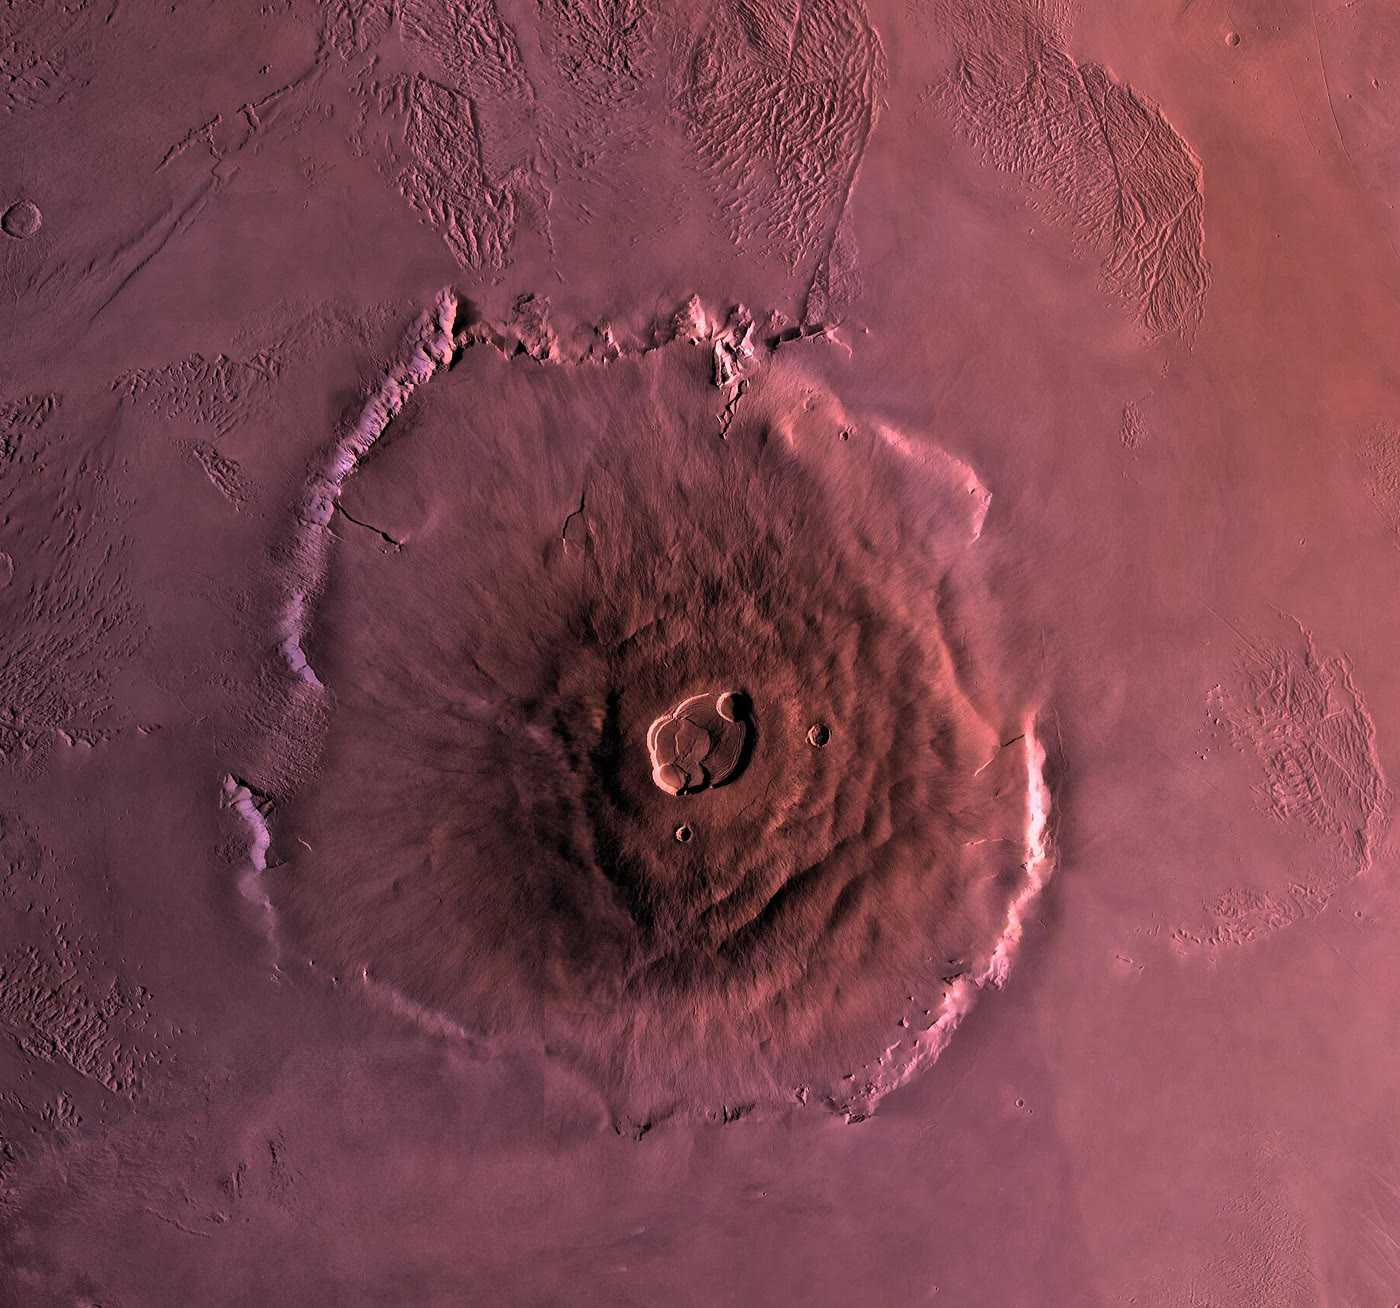
\includegraphics[width=0.48\linewidth]{images/book5/b3-olympus-mons.jpg}
\par\smallskip{\small Olympus Mons en Marte, un mosaico de imágenes de las
sondas orbitales Viking: las calderas de la cumbre en el centro, los flancos de
coladas de lava y el escarpe con acantilados que rodea la base, de unos \qty{600}{km} de diámetro.
NASA/JPL/USGS, dominio público.}\label{fig:b3:planetary-interiors-surfaces:olympus}
\end{omfigure}
% ledger: photo:b3-olympus-mons, nasa:olympus-mons

Venus, gemela de la Tierra en tamaño, tiene con mucho el menor número de cráteres de
impacto de cualquier planeta rocoso salvo la Tierra. Sus rasgos superficiales podrían tener, de media,
una edad de apenas 150 millones de años, con parches más antiguos entre ellos:
el vulcanismo y la deformación renovaron la mayor parte de su superficie, quizá a trozos
a lo largo de mucho tiempo, quizá más deprisa. Venus tiene miles de volcanes y ningún
indicio de placas en movimiento.
% ledger: nasa:venus-surface, planet:Venus.diameter, planet:Earth.diameter

Io, la luna interior más grande de Júpiter, pierde más de
\qty{2.5}{W.m^{-2}} a través de su superficie, unas 27 veces el promedio terrestre
de \qty{0.092}{W.m^{-2}}. Su calor no procede de la radiactividad: lo
generan las mareas.
% ledger: veeder:io-heat, dd10:split

\begin{definition}[Calentamiento de marea]\label{def:b3:planetary-interiors-surfaces:tidal-heating}
El \emph{calentamiento de marea}\index{calentamiento de marea} es el calor producido en el interior de un
cuerpo por la fricción de la deformación que le impone una marea variable.
Una luna en rotación síncrona y órbita excéntrica ve cómo la marea de su planeta
cambia de intensidad y oscila de un lado a otro en cada órbita.
\end{definition}

\begin{proposition}[Potencia de marea de una luna síncrona]\label{prop:b3:planetary-interiors-surfaces:tidal-power}
Una luna de radio $R$ en rotación síncrona, en una órbita de movimiento medio
$n$ y excentricidad pequeña $e$, disipa la potencia
\[
  \dot E = \frac{21}{2}\,\frac{k_2}{Q}\,\frac{(nR)^5}{G}\,e^2 ,
\]
donde $Q$ es el factor de calidad de marea de la luna, de modo que $k_2/Q$ mide
la parte de la deformación de marea que se pierde en forma de calor.
\end{proposition}

La proposición se admite. Las mareas que disipan energía también circularizan
una órbita; la de Io sigue siendo elíptica, de excentricidad 0.004, porque
los tirones de Europa y Ganímedes, sincronizados con gran precisión, la perturban, con
periodos orbitales de 1.77, 3.55 y \num{7.15}~\text{días} que se mantienen casi exactamente en
la razón 1:2:4 (véase el \cref{exo:b3:planetary-interiors-surfaces:8}). Su superficie sube
y baja hasta \qty{100}{m} en cada órbita. Los volcanes
cubren Io de lava más deprisa de lo que se forman cráteres sobre ella; un modelo de
cómo escapa su calor es el \omterm{def:b3:planetary-interiors-surfaces:heat-pipe}{vulcanismo de tubo de calor}, que mantendría una litosfera gruesa y
fría bajo su superficie ardiente.
% ledger: nasa:galilean-orbits, beuthe:tidal-power, nasa:io-orbit, nasa:io-facts

\begin{definition}[Océano subsuperficial]\label{def:b3:planetary-interiors-surfaces:ocean-world}
Un \emph{océano subsuperficial}\index{océano subsuperficial} es una capa global de
agua líquida bajo la capa de hielo de una luna o de un planeta enano, mantenida líquida por
el calor de marea y el radiogénico.
\end{definition}

\begin{definition}[Criovulcanismo]\label{def:b3:planetary-interiors-surfaces:cryovolcanism}
El \emph{criovulcanismo}\index{criovulcanismo} es la erupción de agua, salmueras
u otros líquidos y vapores volátiles, en lugar de roca fundida, sobre la
superficie helada de una luna o de un planeta enano.
\end{definition}

La capa de hielo de Europa, medida por el radiómetro de microondas de la sonda Juno
en la región que sobrevoló, tiene un grosor medio de unos \qty{29}{km}; bajo ella
yace un océano salino que contiene el doble de agua que todos los
océanos de la Tierra. En la luna de Saturno Encélado, de apenas \qty{500}{km}
de diámetro, la sonda Cassini detectó en 2005 chorros de granos de hielo y gas
que escapan por fracturas templadas cerca del polo sur a unos
\qty{400}{m.s^{-1}}. Su gravedad y el balanceo de su rotación mostraron
que los chorros se alimentan de un océano global, bajo una capa de hielo de 20 a
\qty{25}{km} de grosor medio, y quizá de solo 1 a \qty{5}{km} en el
polo sur.
% ledger: jpl:europa-shell, nasa:europa-ocean, nasa:enceladus

\section{Núcleos grandes y pequeños}\label{sec:b3:planetary-interiors-surfaces:cores}

Los cuatro núcleos medidos forman una familia extraña. En relación con su radio, el
núcleo de la Tierra llega al 0.55 del camino hacia la superficie y el de Marte al 0.54; el
de la Luna, al 0.19; el de Mercurio, al 0.82. La diferenciación, en el volumen de segundo año, separa
el metal del silicato dentro de cada cuerpo, pero no puede hacer que las proporciones de
metal sean tan diferentes. Sí pueden hacerlo los impactos gigantes. Se piensa que la Luna se formó
a partir de los escombros de una colisión entre un cuerpo del tamaño de Marte y la
Tierra joven hace unos 4.5 mil millones de años; el metal del impactor se unió
al núcleo de la Tierra y la Luna reunió sobre todo roca del manto, de ahí su
núcleo pequeño. Impactos similares pueden haber despojado de gran parte del manto
silicatado a Mercurio y haberlo dejado como el planeta rico en hierro cuyo núcleo ocupa la mayor parte
de su interior. Los núcleos registran, igual que los cráteres, una historia de colisiones.
% ledger: data:prem, jpl:insight-interior, nasa:moon-core, agu:mercury-core, french:giant-impacts

\section{Ejercicios}

\begin{exercise}[$\star$]\label{exo:b3:planetary-interiors-surfaces:1}
Mercurio tiene una densidad media de \qty{5429}{kg.m^{-3}}, un factor de momento de
inercia de 0.35 y un radio de \qty{2440}{km}. Con un modelo de dos capas y un
manto de \qty{3300}{kg.m^{-3}}, calcúlese el radio relativo del núcleo, su radio en
kilómetros y su densidad.
\end{exercise}

\begin{exercise}[$\star$]\label{exo:b3:planetary-interiors-surfaces:2}
Un proyectil pétreo de \qty{50}{m} de diámetro, de densidad \qty{3500}{kg.m^{-3}},
impacta verticalmente sobre la Tierra a \qty{20}{km.s^{-1}}. Calcúlense su masa y
su energía cinética, en julios y en megatones de explosivo
($\qty{1}{Mt} = \qty{4.2e15}{J}$). ¿Qué diámetro de cráter da la regla
de veinte diámetros del proyectil?
\end{exercise}

\begin{exercise}[$\star$]\label{exo:b3:planetary-interiors-surfaces:3}
En una llanura marciana de \qty{100000}{km^2}, se cuentan 120 cráteres de \qty{1}{km} y
más. Calcúlense $N_1$, su error relativo y la edad modelo de la
llanura con su error.
\end{exercise}

\begin{exercise}[$\star$]\label{exo:b3:planetary-interiors-surfaces:4}
Io, de radio \qty{1821.5}{km}, pierde \qty{2.5}{W.m^{-2}}. Calcúlense su
pérdida de calor total y compárese con la de la Tierra, \qty{47}{TW}, en total y
por metro cuadrado (\qty{0.092}{W.m^{-2}}).
\end{exercise}

\begin{exercise}[$\star\star$]\label{exo:b3:planetary-interiors-surfaces:5}
Marte tiene una masa de \qty{6.417e23}{kg} y un radio de \qty{3389.5}{km}.
(a)~Calcúlense su densidad media, su gravedad superficial y $\rho gR$.
(b)~Tratándolo como una esfera uniforme incompresible de rigidez
\qty{67}{GPa}, calcúlese su \omterm{def:b3:planetary-interiors-surfaces:love-number}{número de Love} $k_2$. (c)~El valor medido es
$0.153 \pm 0.017$. ¿Qué dice la comparación?
\end{exercise}

\begin{exercise}[$\star\star$]\label{exo:b3:planetary-interiors-surfaces:6}
En la Tierra ($g = \qty{9.8}{m.s^{-2}}$), la transición de \omterm{def:b3:planetary-interiors-surfaces:crater-morphology}{cráter simple} a complejo
ocurre a unos \qty{4}{km} en roca cristalina y \qty{2}{km} en
sedimentos. (a)~Suponiendo que el diámetro de la transición varía como $1/g$,
prevéase su valor en la Luna ($g = \qty{1.62}{m.s^{-2}}$) y en Marte y
Mercurio ($g = \qty{3.7}{m.s^{-2}}$); compárese con los \qty{20}{km}
observados en la Luna. (b)~Si el colapso comienza cuando $\rho gD/3$ supera la
resistencia $Y$ de la roca, ¿qué resistencia proporciona la
transición cristalina de la Tierra, para $\rho = \qty{2600}{kg.m^{-3}}$?
\end{exercise}

\begin{exercise}[$\star\star$]\label{exo:b3:planetary-interiors-surfaces:7}
Una superficie tiene $\num{2.0e-3}$ cráteres de \qty{1}{km} o más por
kilómetro cuadrado. Calcúlese su edad modelo con la función de cronología de Marte,
resolviendo la ecuación numéricamente. ¿Qué edad habría dado la función lunar,
y por qué no pueden intercambiarse las dos?
\end{exercise}

\begin{exercise}[$\star\star$]\label{exo:b3:planetary-interiors-surfaces:8}
Los periodos orbitales de Ío, Europa y Ganímedes son 1.769138, 3.551181 y
\num{7.154553}~días. (a)~Calcúlense los cocientes entre periodos sucesivos.
(b)~Calcúlese $1/P_I - 3/P_E + 2/P_G$ y coméntese. (c)~¿Por qué pueden las resonancias
mantener una excentricidad que de otro modo eliminarían las mareas?
\end{exercise}

\begin{exercise}[$\star\star$]\label{exo:b3:planetary-interiors-surfaces:9}
Ío orbita Júpiter en \num{1.769138}~días con excentricidad 0.004.
Calcúlese la potencia que da la proposición sobre potencia de marea por unidad de $k_2/Q$,
y el valor de $k_2/Q$ que suministraría la pérdida de calor de Ío
calculada en el \cref{exo:b3:planetary-interiors-surfaces:4}.
\end{exercise}

\begin{exercise}[$\star\star\star$]\label{exo:b3:planetary-interiors-surfaces:10}
Para la Luna, $\bar\rho = \qty{3340}{kg.m^{-3}}$ y $C = 0.394$.
(a)~Demuéstrese que en el modelo de dos capas $\mathrm dx^2/\mathrm dC =
\tfrac52\bar\rho/(\bar\rho - \rho_m)$ para $\rho_m$ fijo. (b)~Con la
densidad del manto que da un núcleo de $x = 0.19$, \qty{3288}{kg.m^{-3}},
¿cuáles son $x$ y $\rho_c$ cuando $C = 0.395$, y cuando $C = 0.393$?
(c)~¿Qué dice esto sobre la determinación de un núcleo pequeño mediante el momento de
inercia?
\end{exercise}

\begin{exercise}[$\star\star\star$]\label{exo:b3:planetary-interiors-surfaces:11}
(a)~Para 100 cráteres, calcúlese el error de conteo de la edad modelo de una
superficie marciana de \qty{1.0}{Ga} de antigüedad y de otra de \qty{3.8}{Ga}.
(b)~Demuéstrese que en la parte lineal de la función de cronología $\sigma_T/T =
1/\sqrt n$. (c)~¿Por qué siguen siendo inciertas las edades de las superficies antiguas?
\end{exercise}

\begin{exercise}[$\star\star\star$]\label{exo:b3:planetary-interiors-surfaces:12}
Europa, de radio \qty{1560.8}{km}, orbita en \num{3.551181}~días con
excentricidad 0.009. (a)~Si Europa disipara mareas con el mismo $k_2/Q$ que Ío,
¿qué fracción de la potencia de marea de Ío produciría, y qué flujo de calor?
(b)~¿Por qué es dudoso el supuesto para un satélite con un océano bajo su hielo?
\end{exercise}

\section{Problema: dos llanuras en Marte}

\begin{problem}[{Problema de fin de semana --- el núcleo de Marte y las edades de dos
llanuras de lava inventadas}]
\label{pb:b3:planetary-interiors-surfaces:1}
Marte tiene una masa de \qty{6.4169e23}{kg}, un radio de \qty{3389.5}{km} y un
factor de momento de inercia de 0.366. Dos llanuras inventadas, A y B, se encuentran en
sus provincias volcánicas; sus cráteres se han contado en imágenes, agrupados en clases
de anchura $\sqrt2$.

\medskip\noindent\textbf{Parte I --- El núcleo.}
\begin{enumerate}
\item Calcúlese la densidad media de Marte.
\item Con un modelo de dos capas y un manto de \qty{3500}{kg.m^{-3}}, calcúlese
  el radio relativo del núcleo, su radio en kilómetros y su
  densidad.
\item InSight midió un radio del núcleo de \qty{1830}{km}. ¿Qué densidades del manto y del núcleo
  exige entonces el modelo de dos capas?
\item Compárese esa densidad del núcleo con la del núcleo externo de la Tierra
  justo por debajo de su parte superior, \qty{9900}{kg.m^{-3}} en el modelo de Tierra de referencia,
  y explíquese por qué se espera un valor menor para Marte y qué más
  sugiere.
\item El \omterm{def:b3:planetary-interiors-surfaces:love-number}{número de Love} de Marte para una esfera homogénea con una rigidez de
  \qty{67}{GPa} es 0.109; el medido es 0.153. ¿Cuál de las observaciones llegó
  primero, y qué decía ya sobre el núcleo?
\item La corteza de Marte tiene entre 20 y \qty{37}{km} de espesor. ¿Qué fracción del
  volumen del planeta ocupa? ¿Fue correcto ignorarla?
\end{enumerate}

\medskip\noindent\textbf{Parte II --- El recuento de cráteres en la llanura A.} La llanura A
cubre \qty{80000}{km^2}. Sus cráteres, por clase de diámetro (km):
\begin{center}
\small
\begin{tabular}{lccccccccc}
\hline
clase & 1--1.41 & 1.41--2 & 2--2.83 & 2.83--4 & 4--5.66 & 5.66--8 & 8--11.3 & 11.3--16 & 16--22.6 \\
\hline
llanura A & 38 & 6 & 5 & 3 & 0 & 0 & 0 & 1 & 1 \\
llanura B & 48 & 8 & 31 & 12 & 7 & 2 & 0 & 2 & 2 \\
\hline
\end{tabular}
\end{center}
\begin{enumerate}[resume]
\item Calcúlense los recuentos acumulados de la llanura A, a partir de \qty{1}{km}.
\item Calcúlense $N(\qty{1}{km})$ por kilómetro cuadrado y su desviación
  típica.
\item La función de producción da $F(\qty{2}{km}) = 0.147$ y
  $F(\qty{1.41}{km}) = 0.355$. ¿Son los recuentos a 1.41 y \qty{2}{km}
  compatibles con la forma de la función de producción?
\item ¿Está la llanura A siquiera cerca de la densidad de equilibrio,
  \qty{0.072}{km^{-2}} a \qty{1}{km}?
\item ¿Por qué se eligen las clases con anchura $\sqrt2$?
\item Los agrupamientos y cadenas de cráteres pequeños se excluyen de un recuento. ¿Por qué?
\end{enumerate}

\medskip\noindent\textbf{Parte III --- Edades modelo.} Utilícese la
  función de cronología de Marte.
\begin{enumerate}[resume]
\item Calcúlese la edad modelo de la llanura A.
  Compruébese que el término exponencial puede despreciarse.
\item Calcúlese su error de recuento.
\item ¿Qué edad habría dado la cronología lunar?
\item La llanura B cubre \qty{120000}{km^2}. Usando sus cráteres de \qty{2}{km}
  o más, calcúlense $N(\qty{2}{km})$, después $N_1$ y, a continuación, su edad modelo,
  resolviendo la ecuación numéricamente.
\item Calcúlese el error de recuento de esa edad.
\item Compárense los errores relativos de las dos edades y explíquese la
  diferencia.
\end{enumerate}

\medskip\noindent\textbf{Parte IV --- Los cráteres enterrados de la llanura B.}
\begin{enumerate}[resume]
\item ¿Cuántos cráteres entre \num{1} y \qty{2}{km} debería tener la llanura B si
  toda su superficie tuviera la edad de la pregunta~16? ¿Cuántos tiene?
\item Supóngase que la lava enterró todos los cráteres menores de \qty{2}{km} en
  un instante $T_r$ y respetó los mayores. Calcúlese $T_r$ a partir de los
  cráteres de \num{1}--\qty{2}{km}.
\item Calcúlese el error de recuento de $T_r$.
\item Tómese un \omterm{def:b3:planetary-interiors-surfaces:crater-morphology}{cráter simple} fresco en Marte con una profundidad igual a una quinta
  parte de su anchura (supuesto de este problema). ¿Qué espesor debe tener la lava para
  enterrar un cráter de \qty{2}{km}, y por qué siguen apareciendo los mayores?
\item ¿Podrían la lava de la llanura B y la de la llanura A pertenecer a un mismo episodio
  de vulcanismo?
\item Indíquese la edad modelo de la llanura A, en miles de millones de años,
  con dos cifras significativas.
\end{enumerate}
\end{problem}
% ledger: nasa:mars, jpl:insight-interior, yoder:mars-k2, data:prem, craterstats:mars-pf, craterstats:mars-cf, craterstats:moon-cf, craterstats:equilibrium
